%% State Space Modelling of Dynamic Systems
%% Lecture 4: Time Response of a State-Space Model
\def\FileDate{98/10/14}
\def\FileVersion{1.0}
% ----------------------------------------------------------------
% Notes pages *********************************************************
% ----------------------------------------------------------------

Although a state-space model may uniquely represent a given
dynamic system, there is no state-space model that uniquely
represents a given transfer function. That is there are many
state-space models that can be transformed into a given transfer
function. If one begins the analysis of a dynamic system from an
analysis of the elementary dynamics then the state space model
that results from such an analysis will accurately reflect the
physical state variables in the system. However, if one's analysis
begins from a differential equation or (equivalently) from a
transfer function, then it is convenient to transform the model
description into one of a small number of ``standard'' or
\emph{canonical forms}.

\begin{slide}
	\heading{Canonical Forms}
	Standard forms for state space models derived from differential equations or transfer function models.
	\begin{itemize}
		\item Companion form
		\item Controller canonical form
		\item Observer canonical form
		\item Normal form
		\item Jordan forms
	\end{itemize}
\end{slide}



\section*{The Companion Form}
These notes describe how a general differential equation may be
converted into a state-space model.

Consider the general differential equation:

\[
\frac{d^{n}y}{dt^{n}} +
a_{n-1}\frac{d^{n-1}y}{dt^{n-1}}+a_{n-2}\frac{d^{n-2}y}{dt^{n-2}}+\cdots+a_1\frac{dy}{dt}+a_0
y = b_0 u
\]
We rearrange this equation so that the highest power is on the
left
\[
\frac{d^{n}y}{dt^{n}} =
-a_{n-1}\frac{d^{n-1}y}{dt^{n-1}}-a_{n-2}\frac{d^{n-2}y}{dt^{n-2}}-\cdots-a_1\frac{dy}{dt}-a_0
y + b_0 u.
\]
Let:
\begin{eqnarray*}
x_1 &=& y \\ x_2 &=& \frac{dy}{dt} \\ x_3 & = & \frac{d^2y}{dt^2}
\\ \vdots \\ x_{n-1} &=& \frac{d^{n-2}y}{dt^{n-2}} \\ x_{n} &=& \frac{d^{n-1}y}{dt^{n-1}}
\end{eqnarray*}
If we differentiate both sides of these new definitions we obtain
\begin{eqnarray*}
\dot{x}_1 &=& \frac{dy}{dt} \\ \dot{x}_2 &=& \frac{d^2y}{dt^2} \\
\dot{x}_3 & = & \frac{d^3y}{dt^3}
\\ \vdots \\ \dot{x}_{n-1}  &=& \frac{d^{n-1}y}{dt^{n-1}} \\ \dot{x}_{n} &=& \frac{d^{n}y}{dt^{n}}
\end{eqnarray*}

These equations represent the left-hand-side of the state
equations and if we make the substitutions we get
\begin{eqnarray*}
\dot{x}_1 &=&
   x_2 \\ \dot{x}_2 &=&  x_3   \\
\dot{x}_3 & = &  x_4
\\ \vdots \\ \dot{x}_{n-1}  &=& x_n \\ \dot{x}_{n} &=&
-a_{0}x_1 -a_1x_2 - \cdots  -a_{n-2}x_{n-1} -a_{n-1}x_{n} + b_0 u
\end{eqnarray*}
We then define the state vector \[\mathbf{x}=[x_1,\ x_2,\ \ldots,\
x_n]^T\] and the matrix form of the state equations are
\[
\dot{\mathbf{x}} = \left[\begin{array}{ccccc}
  0 & 1 & 0 & \cdots & 0 \\
  0 & 0 & 1 & \cdots & 0 \\
  \vdots & \vdots & \vdots & \ddots & \vdots \\
  0 & 0 & 0 & \cdots & 1 \\
  -a_{0} & -a_{1} & -a_{2} & \cdots & -a_{n-1}
\end{array}\right]\mathbf{x}+\left[\begin{array}{c}
  0 \\
  0 \\
  0 \\
  \vdots \\
  1
\end{array}\right]u
\]
The system matrix is in ``\emph{companion form}'', so called because the
coefficients in the final row are the same as for the differential
equation. The output equation depends on the dependent variable of
interest but the simplest is $y=x_1$ which gives the solution of
the differential equation. Thus
\[y = [1,\ 0,\ 0,\ \ldots, 0] \mathbf{x}.\]

The transfer function equivalent of this differential equation is
obtained from the differential equation:
\[
\frac{d^{n}y}{dt^{n}} +
a_{n-1}\frac{d^{n-1}y}{dt^{n-1}}+a_{n-2}\frac{d^{n-2}y}{dt^{n-2}}+\cdots+a_1\frac{dy}{dt}+a_0
y = b_0 u
\]
The transform of this equation, ignoring initial conditions, is
\[
\left(s^n +
a_{n-1}s^{n-1}+a_{n-2}s^{n-2}+\cdots+a_1s+a_0\right)Y(s) = b_0
U(s)
\]
so the transfer function is
\[
G(s) = \frac{Y(s)}{U(s)} = \frac{b_0}{s^n +
a_{n-1}s^{n-1}+a_{n-2}s^{n-2}+\cdots+a_1s+a_0}.
\]
Note that the numerator has no terms in $s$. We shall consider
completely general case for both proper and strictly proper
systems later.

\section*{The Companion Form}

We have just shown that a state space model
for the system defined by the general differential equation, shown
in \sref{slide:l5s1}, was the companion form illustrated in
\sref{slide:l5s2}. This structure of this state-space model is
illustrated in \sref{slide:l5s3}.
\begin{slide}\label{slide:l5s1}
\heading{General Differential Equation}
\[ \frac{d^{n}y}{dt^{n}} +
a_{n-1}\frac{d^{n-1}y}{dt^{n-1}}+a_{n-2}\frac{d^{n-2}y}{dt^{n-2}}+\cdots+a_1\frac{dy}{dt}+a_0
y = b_0 u
\]
or transfer function
\[
G(s) = \frac{Y(s)}{U(s)} = \frac{b_0}{s^n +
a_{n-1}s^{n-1}+a_{n-2}s^{n-2}+\cdots+a_1s+a_0}.
\]
The state variables in this model are the so-called ``\emph{phase
variables}'' $x_1 = y$, $x_2 = dy/dt$, $\ldots$ $x_n = d^n/dt^n$.
\end{slide}
\begin{slide}\label{slide:l5s2}
\heading{Companion Form}
\begin{eqnarray*} \dot{\mathbf{x}} &=&
\left[\begin{array}{ccccc}
  0 & 1 & 0 & \cdots & 0 \\
  0 & 0 & 1 & \cdots & 0 \\
  \vdots & \vdots & \vdots & \ddots & \vdots \\
  0 & 0 & 0 & \cdots & 1 \\
  -a_{0} & -a_{1} & -a_{2} & \cdots & -a_{n-1}
\end{array}\right]\mathbf{x}+\left[\begin{array}{c}
  0 \\
  0 \\
  0 \\
  \vdots \\
  b_0
\end{array}\right]u\\
y & = & [1,\ 0,\ 0,\ \ldots, 0] \mathbf{x}.
\end{eqnarray*}
\end{slide}
\begin{slide}\label{slide:l5s3}
\heading{Block Diagram of Companion Form}
\resizebox{300pt}{!}{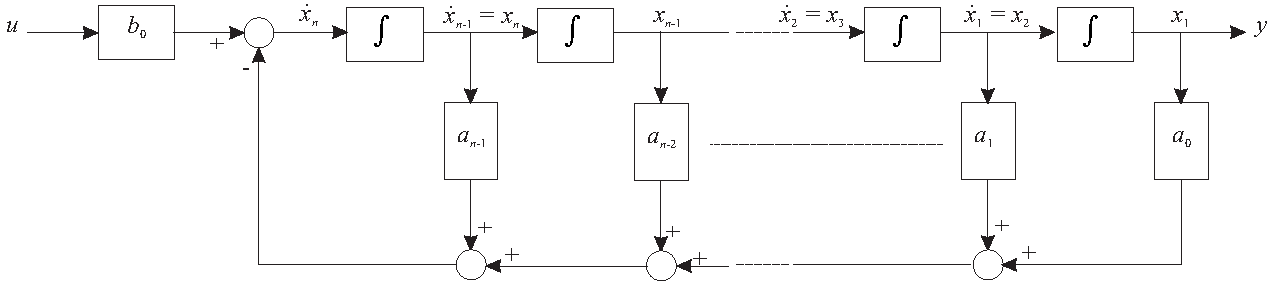
\includegraphics{pictures/companion1.pdf}}
\end{slide}

Now let us consider the case of a system that has derivatives of
the input. A strictly proper system has transfer function
\[G(s)=\frac{Y(s)}{U(s)} = \frac{b_ms^m +
b_{m-1}s^{m-1}+b_{m-2}s^{m-2}+\cdots+b_1s+b_0}{s^n +
a_{n-1}s^{n-1}+a_{n-2}s^{n-2}+\cdots+a_1s+a_0}\] where $m<n$. How
is this more general system converted into a state-space model?
Well, from the previous result let us use the state definition
$x_1(t) = y(t)$ to split the transfer function so that
\begin{equation}\label{eq:l5e1}
X_1(s) = \frac{1}{s^n +
a_{n-1}s^{n-1}+a_{n-2}s^{n-2}+\cdots+a_1s+a_0}U(s)
\end{equation}
and
\begin{equation}\label{eq:l5e2}
Y(s) = \left(b_ms^m +
b_{m-1}s^{m-1}+b_{m-2}s^{m-2}+\cdots+b_1s+b_0\right)X_1(s).\end{equation}
Inverse Laplace transforming equation (\ref{eq:l5e2}) we get:
\begin{eqnarray}\label{eq:l5e3}
y(t) & = & b_m\frac{d^m}{dt^m}x_1(t) +
b_{m-1}\frac{d^{m-1}}{dt^{m-1}}x_1(t)+\cdots+b_1\frac{d}{dt}x_1(t)+
b_0x_1(t)\\ & = & b_mx_{m+1}(t) + b_{m-1}x_m(t)+\cdots+b_1x_2(t)+
b_0x_1(t).\label{eq:l5e4}
\end{eqnarray}
Where, in (\ref{eq:l5e4}), substitutions have been made according
to the definition of the phase variables. The vector state
equations are therefore: \begin{eqnarray*} \dot{\mathbf{x}} &=&
\left[\begin{array}{ccccc}
  0 & 1 & 0 & \cdots & 0 \\
  0 & 0 & 1 & \cdots & 0 \\
  \vdots & \vdots & \vdots & \ddots & \vdots \\
  0 & 0 & 0 & \cdots & 1 \\
  -a_{0} & -a_{1} & -a_{2} & \cdots & -a_{n-1}
\end{array}\right]\mathbf{x}+\left[\begin{array}{c}
  0 \\
  0 \\
  0 \\
  \vdots \\
  1
\end{array}\right]u\\
y & = & [b_0,\ b_1,\ \dots,\ b_{m-1}, b_m]
\mathbf{x}.\end{eqnarray*} Note that the coefficients of the
numerator appear in reverse order in the $\mathbf{C}$ matrix. The
structure of this system is illustrated in \sref{slide:l5s4} for
the case $m=n-1$.
\begin{slide}\label{slide:l5s4}
\heading{Strictly Proper Companion Form}
\resizebox{300pt}{!}{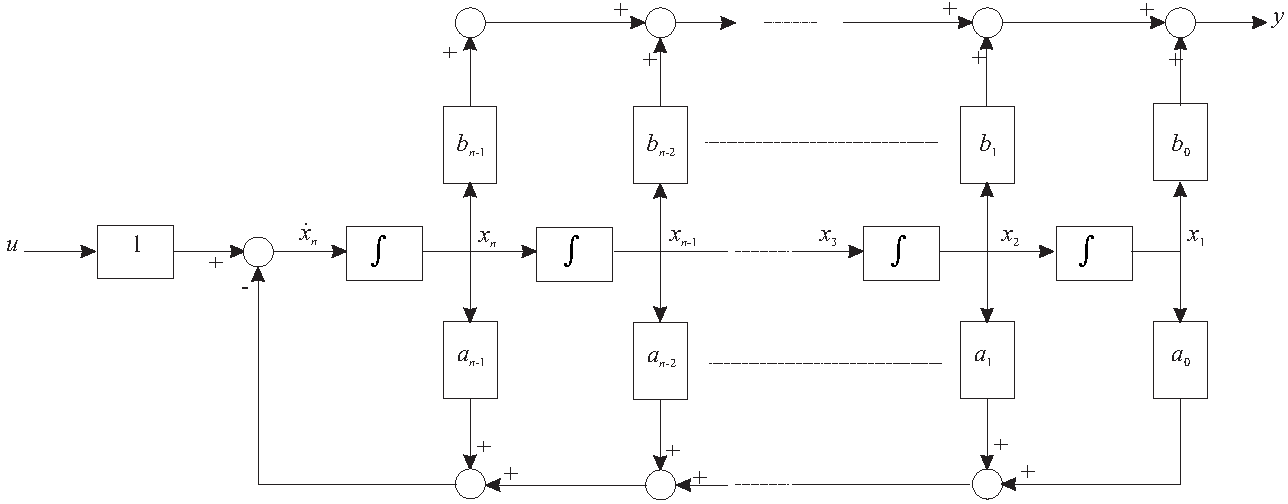
\includegraphics{pictures/companion2.pdf}}
\end{slide}

The general form of a transfer function of a proper single-input,
single-output system of order $n$ is
\[\frac{b_ns^n+b_{n-1}s^{n-1}+\cdots+b_1s + b_0}{s^n+a_{n-1}s^{n-1}+\cdots+a_1s + a_0}\]
An alternative form, obtained by dividing the numerator by the
denominator, is
\[b_n+\frac{(b_{n-1}-b_n)s^{n-1}+\cdots+(b_1-b_n)+(b_0-b_n)}{s^n+a_{n-1}s^{n-1}+\cdots+a_1s + a_0}.\]
If we define $d=b_n$ and the modified numerator coefficients are
\[c_j=b_j-b_n,\ j=1,2,\ldots,n\] then the transfer function may be
re-written
\[d+\frac{c_{n-1}s^{n-1}+c_{n-2}s^{n-2}+\cdots+c_1s + c_n}{s^n+a_{n-1}s^{n-1}+\cdots++a_1s + a_0}.\]
Writing the transfer function in its functional form we have:
\[Y(s)=d U(s) +\frac{c_{n-1}s^{n-1}+c_{n-2}s^{n-2}+\cdots+c_1s +
c_n}{s^n+a_{n-1}s^{n-1}+\cdots+a_1s + a_0}U(s).\] Performing a
similar analysis, as before, we obtain the state-equations for a
proper system:
\begin{eqnarray*}\dot{\mathbf{x}} & = & \left[\begin{array}{ccccc}
  0 & 1 & 0 & \cdots & 0 \\
  0 & 0 & 1 & \cdots & 0 \\
  \vdots & \vdots & \vdots & \ddots & \vdots \\
  0 & 0 & 0 & \cdots & 1 \\
  -a_{0} & -a_{1} & -a_{2} & \cdots & -a_{n-1}
\end{array}\right]\mathbf{x}+\left[\begin{array}{c}
  0 \\
  0 \\
  0 \\
  \vdots \\
  1
\end{array}\right]u\\
y & = & [c_0,\ c_1,\ \dots,\ c_{m-1}, c_m] \mathbf{x} + d
u.\end{eqnarray*} The block diagram fro this system is illustrated
in \sref{slide:proper}.
\begin{slide}\label{slide:proper}
\heading{Proper System: Block Diagram}
\resizebox{320pt}{!}{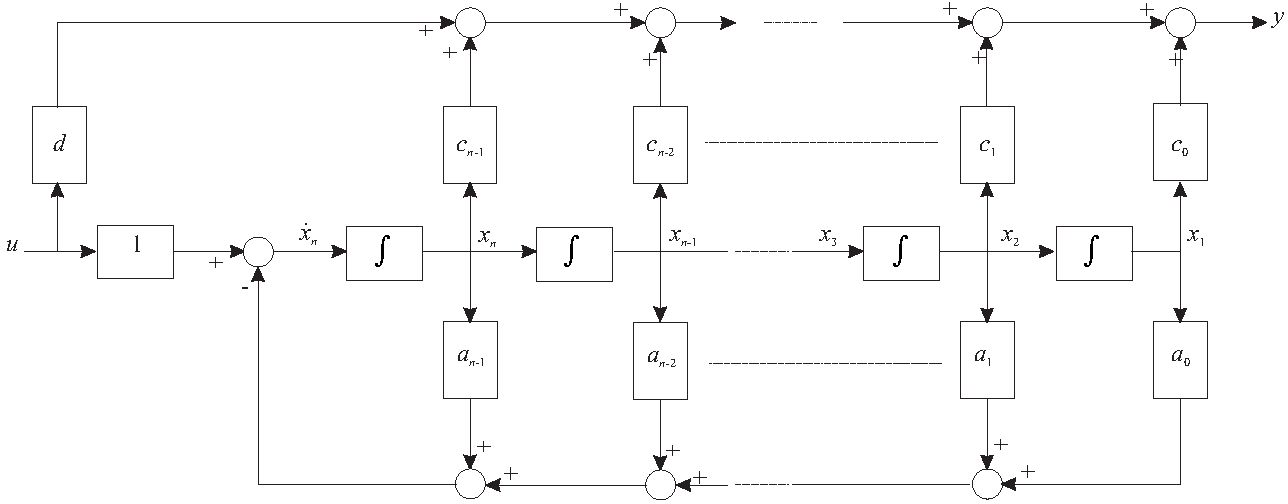
\includegraphics{pictures/companion3.pdf}}
\end{slide}


\section*{Example}

\begin{slide}
\heading{Example}
System with transfer function
\[G(s)=\frac{Y(s)}{U(s)}=\frac{2s^3 + 16s^2 + 30s + 8}{s^3 + 7s^2 + 10s}\]
This system is ``proper'' because order of numerator equals order of denominator.
\end{slide}
\begin{slide}
\heading{Example (2)}
First divide the numerator into the denominator to get
\begin{eqnarray*}G(s)&=&\frac{2(s^3 + 7s^2 + 10s) + 2s^2 + 10s + 8}{s^3 + 7s^2 +
10s}\\ &=& \frac{2s^2 + 10s + 8}{s^3 + 7s^2 + 10s} +
2.\end{eqnarray*} 
\end{slide}
\begin{slide}
\heading{Example (completed)}
The companion form of the state matrices are
\begin{eqnarray*}\mathbf{A} & = & \left[\begin{array}{ccc}
  0 & 1 & 0 \\
  0 & 0 & 1 \\
  0 & -10 & -7
\end{array}\right]\ \mathbf{B}=\left[\begin{array}{c}
  0 \\
  0 \\
  1
\end{array}\right]\\ \mathbf{C} & = & \left[\begin{array}{ccc}
  8 & 10 & 2
\end{array}\right]\ \mathbf{D}=\left[2\right]\end{eqnarray*}
\end{slide}

%% State Space Modelling of Dynamic Systems
%% Normal Canonical Form
\def\FileDate{98/11/03}
\def\FileVersion{1.0}
% ----------------------------------------------------------------
% Notes pages *********************************************************
% ----------------------------------------------------------------

\section*{Controller Canonical Form}
If one defines a transfer function in \Matlab{}, e.g. as shown in
\sref{slide:l5s5}, the result of converting the system into
state-space form is rather surprisingly not the companion form we
have seen before. Instead, the result is what is known as the
\emph{Controller Canonical Form}. This is still a companion form
because the coefficients of the $\mathbf{A}$ and $\mathbf{C}$
matrices are the coefficients of the transfer function's
denominator and numerator polynomials.
\begin{slide}\label{slide:l5s5}\heading{A Little \Matlab{}}
Let \[ G(s)
=\frac{Y(s)}{U(s)} = \frac{s^2 + 7s + 2 }{s^3 + 9s^2 + 26s + 24}\]
\begin{verbatim}
>> num=[1, 7, 2]; den=[1, 9, 26 24];
>> [A,B,C,D]=tf2ss(num,den);
\end{verbatim}
Result:
\begin{eqnarray*}
\dot{\mathbf{x}} & = &\left[\begin{array}{ccc}
  -9 & -26 & -24  \\
  1 & 0 & 0  \\
  0 & 1  & 0
 \end{array}\right]\mathbf{x}+\left[\begin{array}{c}
  1 \\
  0 \\
  0
\end{array}\right]u\\
y & = & [1,\ 7,\ 2] \mathbf{x}.\end{eqnarray*}
\end{slide}
The controller canonical form is simply obtained by re-ordering
the phase variables as shown in \sref{slide:l5s6},
\sref{slide:l5s6-2} and \sref{slide:l5s7}. The general form of the
controller canonical state-space model is as shown in
\sref{slide:l5s8}.
\begin{slide}
\label{slide:l5s6} \heading{Companion Form}
\begin{eqnarray*} \left[\begin{array}{c}
  \dot{x}_{1} \\
  \dot{x}_{2} \\
  \vdots \\
  \dot{x}_{n-1} \\
  \dot{x}_n
\end{array}\right] &=& \left[\begin{array}{ccccc}
  0 & 1 & 0 & \cdots & 0 \\
  0 & 0 & 1 & \cdots & 0 \\
  \vdots & \vdots & \vdots & \ddots & \vdots \\
  0 & 0 & 0 & \cdots & 1 \\
  -a_{0} & -a_{1} & -a_{2} & \cdots & -a_{n-1}
\end{array}\right]\left[\begin{array}{c}
  {x}_{1} \\
  {x}_{2} \\
  \vdots \\
  {x}_{n-1} \\
  {x}_{n}
\end{array}\right]+\left[\begin{array}{c}
  0 \\
  0 \\
  \vdots \\
  0 \\
  1
\end{array}\right]u\\
y & = & [b_0,\ b_1,\ \dots,\ b_{n-2}, b_{n-1}][
  {x}_{1},\
  {x}_{2},\
  \ldots,\
  {x}_{n-1},\
  {x}_{n}]^T
\end{eqnarray*}
\end{slide}
\begin{slide}\label{slide:l5s6-2}
\heading{Controller canonical form: Re-number States}

\begin{eqnarray*} \left[\begin{array}{c}
  \dot{x}_{n} \\
  \dot{x}_{n-1} \\
  \vdots \\
  \dot{x}_{2} \\
  \dot{x}_{1}
\end{array}\right] &=& \left[\begin{array}{ccccc}
  0 & 1 & 0 & \cdots & 0 \\
  0 & 0 & 1 & \cdots & 0 \\
  \vdots & \vdots & \vdots & \ddots & \vdots \\
  0 & 0 & 0 & \cdots & 1 \\
  -a_{0} & -a_{1} & -a_{2} & \cdots & -a_{n-1}
\end{array}\right]\left[\begin{array}{c}
  {x}_{n} \\
  {x}_{n-1} \\
  \vdots \\
  {x}_{2} \\
  {x}_{1}
\end{array}\right]+\left[\begin{array}{c}
  0 \\
  0 \\
  \vdots \\
  0 \\
  1
\end{array}\right]u\\ y & = & [b_0,\ b_1,\ \dots,\ b_{n-2}, b_{n-1}]
\left[
  {x}_{n},\
  {x}_{n-1},\
  \ldots,\
  {x}_{2},\
  {x}_{1}
\right]^T
\end{eqnarray*}
\end{slide}
\begin{slide}\label{slide:l5s7}
\heading{Controller canonical form: Re-Ordered States}

\begin{eqnarray*} \left[\begin{array}{c}
  \dot{x}_{1} \\
  \dot{x}_{2} \\
  \vdots \\
  \dot{x}_{n-1} \\
  \dot{x}_{n}
\end{array}\right] &=& \left[\begin{array}{ccccc}
 -a_{n-1} & -a_{n-2} & \cdots & -a_{1} & -a_{0} \\
   1 & 0 & \cdots & 0 & 0 \\
  0 & 1 & \cdots & 0 & 0 \\
  \vdots & \vdots & \ddots & \vdots & \vdots \\
  0 & 0 & \cdots & 1 & 0
\end{array}\right]\left[\begin{array}{c}
  {x}_{1} \\
  {x}_{2} \\
  \vdots \\
  {x}_{n-1} \\
  {x}_{n}
\end{array}\right]+\left[\begin{array}{c}
  1 \\
  0 \\
  \vdots \\
  0 \\
  0
\end{array}\right]u\\ y & = & [b_{n-1},\ b_{n-2},\ \dots,\ b_{1}, b_{0}]
\left[
  {x}_{1},\
  {x}_{2},\
  \ldots,\
  {x}_{n-1},\
  {x}_{n}
\right]^T
\end{eqnarray*}
\end{slide}
\begin{slide}
\label{slide:l5s8} \heading{Controller Canonical Form: Block
Diagram} \resizebox{300pt}{!}{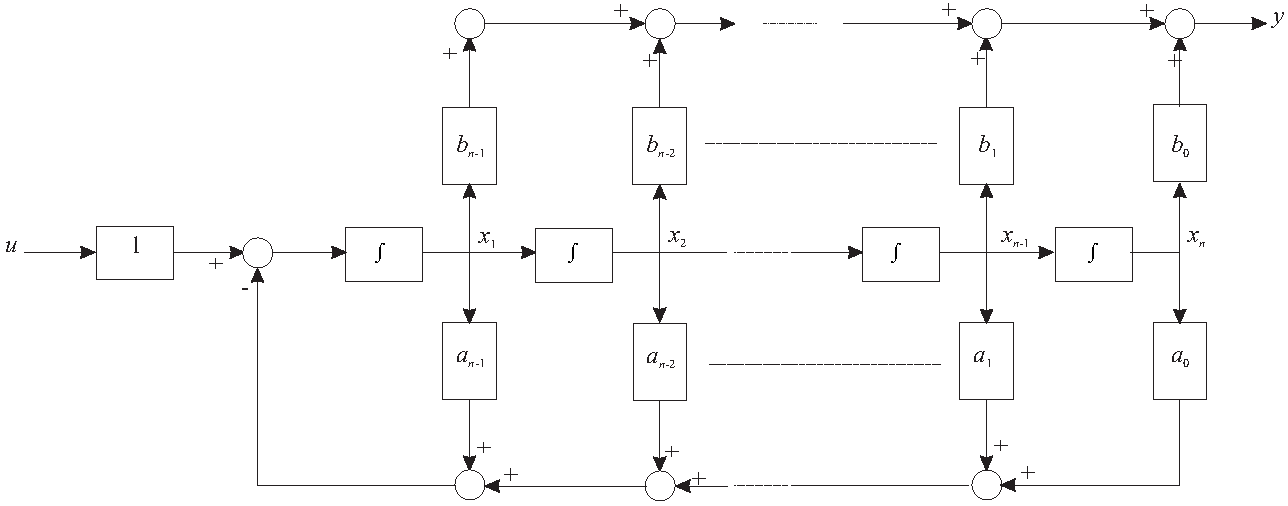
\includegraphics{pictures/ccanon.pdf}}
\end{slide}

\section*{Observer Canonical Form}
The observer canonical form is the "dual" of the controller
canonical form. The state equations are shown in
\sref{slide:l5s9}. Note that the $\mathbf{A}$ matrix is the
transpose of the controller canonical form and that $\mathbf{b}$
and $\mathbf{c}$ are the transposes of the $\mathbf{c}$ and
$\mathbf{b}$ matrices, respectively, of the controller canonical
form.
\begin{slide} \label{slide:l5s9} \heading{Observer Canonical Form}
\begin{eqnarray*} \left[\begin{array}{c}
  \dot{x}_{n} \\
  \dot{x}_{n-1} \\
  \vdots \\
  \dot{x}_{2} \\
  \dot{x}_{1}
\end{array}\right] &=& \left[\begin{array}{ccccc}
 -a_{n-1} & 1 & 0 & \cdots & 0 \\
 -a_{n-2} & 0 & 1 & \cdots & 0 \\
 -a_{n-3} & 0 & 0 & \cdots & 0 \\
  \vdots & \vdots & \vdots & \ddots & \vdots \\
 -a_{1} & 0 & \cdots & 0 & 1 \\
 -a_{0} & 0 & \cdots & 0 & 0
\end{array}\right]\left[\begin{array}{c}
  {x}_{1} \\
  {x}_{2} \\
  {x}_{3} \\
  \vdots \\
  {x}_{n-1} \\
  {x}_{n}
\end{array}\right]+\left[\begin{array}{c}
  b_{n-1} \\
  b_{n-2} \\
  b_{n-3} \\
  \vdots \\
  b_{1} \\
  b_0
\end{array}\right]u\\ y & = & [1,\ 0,\ 0,\ \ldots, 0]\left[
  {x}_{1},\
  {x}_{2},\
  \ldots,\
  {x}_{n-1},\
  {x}_{n}
\right]^T
\end{eqnarray*}
\end{slide}
\begin{slide}
\label{slide:l5s} \heading{Observer Canonical Form: Block Diagram}
\resizebox{300pt}{!}{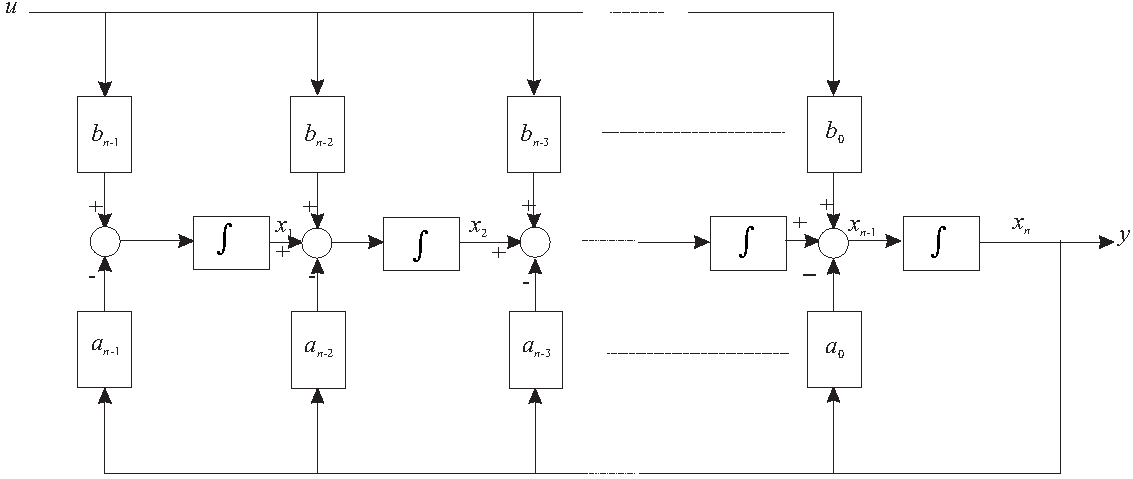
\includegraphics{pictures/ocanon.pdf}}
\end{slide}

\section*{Examples of Companion Forms}
The system with transfer function
\[G(s)=\frac{Y(s)}{U(s)}=\frac{2s^3 + 16s^2 + 30s + 8}{s^3 + 7s^2 + 10s}\]
was found, in the last lecture, to have companion form
\begin{eqnarray*}\mathbf{A} & = & \left[\begin{array}{ccc}
  0 & 1 & 0 \\
  0 & 0 & 1 \\
  0 & -10 & -7
\end{array}\right]\ \mathbf{B}=\left[\begin{array}{c}
  0 \\
  0 \\
  1
\end{array}\right]\\ \mathbf{C} & = & \left[\begin{array}{ccc}
  8 & 10 & 2
\end{array}\right]\ \mathbf{D}=\left[2\right]\end{eqnarray*}
The controller canonical form is obtained by re-ordering the state
variables:
\begin{eqnarray*}\mathbf{A} & = & \left[\begin{array}{ccc}
  -7 & -10 & 0 \\
  1 & 0 & 0 \\
  0 & 1 & 0
\end{array}\right]\ \mathbf{B}=\left[\begin{array}{c}
  1 \\
  0 \\
  0
\end{array}\right]\\ \mathbf{C} & = & \left[\begin{array}{ccc}
  2 & 8 & 10
\end{array}\right]\ \mathbf{D}=\left[2\right]\end{eqnarray*}
and the observable canonical form is obtained by transposing the
$\mathbf{A}$ matrix and letting $\mathbf{B} = \mathbf{C}^T$ and
$\mathbf{C}=\mathbf{B}^T$.
\begin{eqnarray*}\mathbf{A} & = & \left[\begin{array}{ccc}
  -7 & 1 & 0 \\
  -10 & 0 & 1 \\
  0 & 0 & 0
\end{array}\right]\ \mathbf{B}=\left[\begin{array}{c}
  2 \\
  8 \\
  10
\end{array}\right]\\ \mathbf{C} & = & \left[\begin{array}{ccc}
  1 & 0 & 0
\end{array}\right]\ \mathbf{D}=\left[2\right]\end{eqnarray*}
\begin{slide}\label{slide:l5s10}
\heading{\Matlab{} Code for Example}
\begin{verbatim}
>> num = [2, 16, 30, 8]; den = [1, 7, 10, 0];
>> G = tf(num,den);
>> Gcc = ss(G);
>> [Acc,Bcc,Ccc,Dcc]=ssdata(Gcc);
\end{verbatim}
The resulting variables \verb|A|, \verb|B|, \verb|C|, and \verb|D|
are in controller canonical form.
\begin{verbatim}
>> Goc = ss(Acc',Ccc',Bcc',Dcc);
\end{verbatim}
will create the observer canonical form.
\end{slide}
\begin{slide}\label{slide:15s10a}
\heading{$\ldots$ Companion Form}
To obtain the companion form,
some \Matlab{} trickery is needed to re-order the controller
canonical state matrices:
\begin{verbatim}
>> [n,m]=size(Acc); % n = m = 3 for the example
>> Acf = Acc(n:-1:1,n:-1:1);
>> Bcf = Bcc(n:-1:1,:); 
>> Ccf = Ccc(:,n:-1:1);
>> Dcf = Dcc;
\end{verbatim}
The companion form is then created from the reordered matrices.
\begin{verbatim}
>> Gcf = ss(Acf,Bcf,Ccf,Dcf);
\end{verbatim}
\end{slide}
\begin{slide}\label{slide:l5s11}
\heading{\emph{All Forms} Represent the Same Transfer Function!}
\begin{verbatim}
>> G1 = tf(Gcf) % Companion form
Transfer function:
2 s^3 + 16 s^2 + 30 s + 8
-------------------------
   s^3 + 7 s^2 + 10 s
>> G2 = tf(Gcc) % Controller Canonical form
ditto!
>> G3 = tf(Goc) % Observer Canonical Form
ditto!
\end{verbatim}
\end{slide}
We now consider one
final canonical form, the so-called ``normal'' or ``parallel''
form.

\section*{Normal Canonical Form}
The normal form of
a state-space model isolates the characteristic values, also
called the eigen values, or system poles, of the system.

If all the poles of a system are real and distinct then the
transfer function may be written as a partial fraction expansion
\[ G(s) = \frac{Y(s)}{U(s)} = \left\{\frac{r_1}{s-p_1} +
\frac{r_2}{s-p_2} + \cdots + \frac{r_n}{s-p_n} + d\right\}
\]
we can develop a state-space model for each term:
\[Y(s)=\frac{r_i}{s-p_i}U(s).\]
\begin{eqnarray*}
(s-p_i)Y(s) & = & r_i U(s)\\ \frac{d}{dt}y(t)-p_i y(t) &=& r_i
u(t).\end{eqnarray*} If we let $x_i(t) = y(t)$ then
\begin{eqnarray*}
\dot{x}_i &=& p_i x_i + r_i u \\ y &=& x_i
\end{eqnarray*}
Thus, each partial fraction term may be represented by the block
diagram shown in \sref{slide:l6s1}.
\begin{slide}\label{slide:l6s1}
\heading{State-Space Model of $\frac{r_i}{s-p_i}$}
\begin{eqnarray*}
\dot{x}_i &=& p_i x_i + r_i u \\ y &=& x_i
\end{eqnarray*}
\resizebox{300pt}{!}{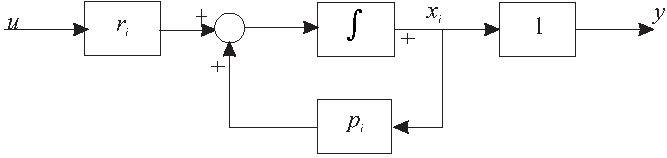
\includegraphics{pictures/sspole.pdf}}
\end{slide}
Thus, the total state-space model of the system is simply the sum
of such terms as shown in \sref{slide:l6s2}.
\begin{slide}\label{slide:l6s2}
\heading{Normal Canonical Form: Block Diagram}
\resizebox{300pt}{!}{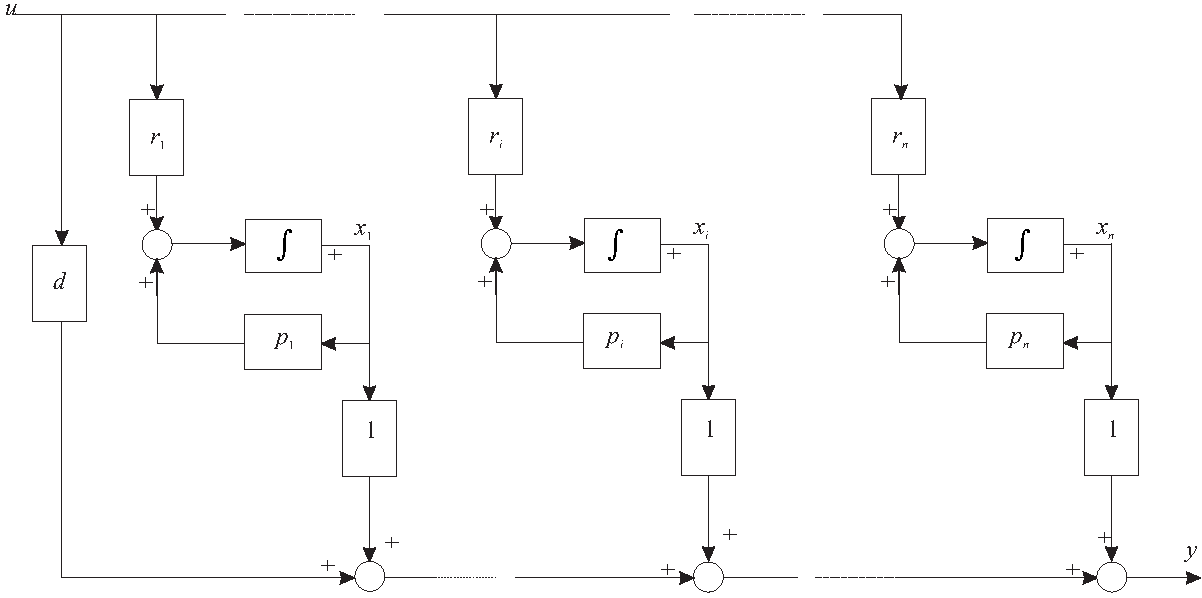
\includegraphics{pictures/normalcan.pdf}}
\end{slide}

Therefore the state space model for the whole system is as shown
in \sref{slide:l6s3}.
\begin{slide}\label{slide:l6s3}
\heading{Normal Observable Canonical State Space Model}
\begin{eqnarray*} \mathbf{\dot{x}}&=&\left[\begin{array}{ccccc}
  p_1 & 0 & 0 & \cdots & 0 \\
  0 & p_2 & 0 & \cdots & 0 \\
  0 & 0 & p_3 & \cdots & 0 \\
  \vdots & \vdots & \vdots & \ddots & \vdots \\
  0 & 0 & 0 & \cdots & p_n
\end{array}\right] \mathbf{x} + \left[\begin{array}{c}
  r_1 \\
  r_2 \\
  r_3 \\
  \vdots \\
  r_n
\end{array}\right] u\\ y &=& \left[1,\ 1,\ 1,\ \ldots,\ 1\right] \mathbf{x} + d u
\end{eqnarray*}
 \end{slide}

Note that the residues of the partial fraction expansion $r_1,\
r_2,\ \ldots,\ r_n$ have been allocated to the input side of the
block diagram and therefore to the input matrix in the state space
model. This model, in which all the elements of the output matrix
are unity, is called the ``\emph{Normal Observable Canonical
Form}''. It would be equally valid to allocate the residues to the
output matrix, leaving the elements of the input matrix as unity,
this would be the ``\emph{Normal Controllable Canonical Form}''
illustrated in \sref{slide:l6s3b}.

\begin{slide}\label{slide:l6s3b}
\heading{Normal Controllable Canonical State Space Model}
\begin{eqnarray*} \mathbf{\dot{x}}&=&\left[\begin{array}{ccccc}
  p_1 & 0 & 0 & \cdots & 0 \\
  0 & p_2 & 0 & \cdots & 0 \\
  0 & 0 & p_3 & \cdots & 0 \\
  \vdots & \vdots & \vdots & \ddots & \vdots \\
  0 & 0 & 0 & \cdots & p_n
\end{array}\right] \mathbf{x} + \left[\begin{array}{c}
  1 \\
  1 \\
  1 \\
  \vdots \\
  1
\end{array}\right] u\\ y &=& \left[r_1,\ r_2,\ r_3,\ \ldots,\ r_n\right] \mathbf{x} + d u
\end{eqnarray*}
 \end{slide}

The most important property of the normal canonical model is that
the $\mathbf{A}$ matrix is diagonal and that the elements on the
diagonal are the eigenvalues of the system matrix. If you form the
system transition matrix for this system each state response is
simply of the form $r_i e^{p_i t}$, that is each state response is
equal to the corresponding mode response\footnote{The proof is
left as an exercise.}.

\subsection*{Example}
For the system examined earlier
\begin{eqnarray*}
G(s) &=& \frac{2s^3 + 16s^2 + 30s + 8}{s^3 + 7s^2 + 10s} \\
 &=&
\frac{2s^2 + 10s + 8}{s^3 + 7s^2 + 10s} + 2 \\
 &=& \frac{2s^2 + 10s + 8}{s(s+2)(s+5)} + 2 \\
 &=& \frac{4/5}{s} + \frac{2/3}{s+2} + \frac{8/15}{s+5} + 2
\\
\end{eqnarray*}
The normal controllable canonical form therefore is:
\begin{eqnarray*}
\mathbf{\dot{x}}&=&\left[\begin{array}{ccc}
  0 & 0 & 0  \\
  0 & -2 & 0  \\
  0 & 0 & -5  \\
 \end{array}\right] \mathbf{x} + \left[\begin{array}{c}
  4/5 \\
  2/3 \\
  8/15
\end{array}\right] u\\ y &=& \left[1,\ 1,\ 1\right] \mathbf{x} + d u
\end{eqnarray*}
and the normal observable canonical form is:
\begin{eqnarray*}
\mathbf{\dot{x}}&=&\left[\begin{array}{ccc}
  0 & 0 & 0  \\
  0 & -2 & 0  \\
  0 & 0 & -5  \\
 \end{array}\right] \mathbf{x} + \left[\begin{array}{c}
  1 \\
  1  \\
  1
\end{array}\right] u\\ y &=& \left[4/5,\ 2/3,\ 8/15\right] \mathbf{x} + d u
\end{eqnarray*}

\subsection*{Time Response from Normal Form}

Notice that in the case of a system defined in \emph{normal form}, because the $\mathbf{A}$ matrix is diagonal, the state equations are decoupled from each other and can be solved independently. This canonical form is useful for the solution of the state equations. Thus given initial states $x_1(t)=x_{10}$, $x_2(t)=x_{20}$, etc at $t=0$ and taking Laplace transforms of the first row of the state equations derived above, the solutions are:
\begin{eqnarray*}
 sX_1 (s) - x_{10}  & = & p_1 X_1 (s) + r_1 U(s) \\ 
 (s - p_1 )X_1 (s) & = & x_{10}  + r_1 U(s) \\ 
 X_1 (s) & = & \frac{{x_{10} }}{{s - p_1 }} + \frac{{r_1 }}{{s - p_1 }}U(s)
\end{eqnarray*}
Taking inverse Laplace transforms:
\[ x_1 = x_{10}e^{p_1t}+r_1\int_0^tu(\tau)e^{p_1(t-\tau)}d\tau \]
and similarly for the other states.
\ifslidesonly
\begin{slide}
	\heading{Time response from Normal Form}
	Given initial states $x_1(t)=x_{10}$, $x_2(t)=x_{20}$, etc at $t=0$
	\begin{eqnarray*}
	 sX_1 (s) - x_{10}  & = & p_1 X_1 (s) + r_1 U(s) \\ 
	 (s - p_1 )X_1 (s) & = & x_{10}  + r_1 U(s) \\ 
	 X_1 (s) & = & \frac{{x_{10} }}{{s - p_1 }} + \frac{{r_1 }}{{s - p_1 }}U(s)
	\end{eqnarray*}
	Taking inverse Laplace transforms:
	\[ x_1 = x_{10}e^{p_1t}+r_1\int_0^tu(\tau)e^{p_1(t-\tau)}d\tau \]
	Repeated for the other states.
\end{slide}
\fi

These are then combined through the output equation to give the solution for $y$:

\begin{center}
	\resizebox{200pt}{!}{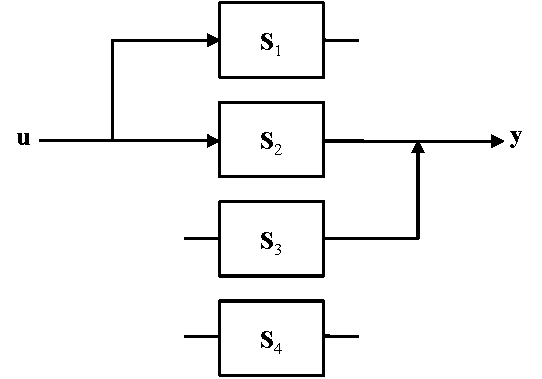
\includegraphics{pictures/partitioning.pdf}}
\end{center}
\endinput

%%% Local Variables: 
%%% mode: latex
%%% TeX-master: "notes"
%%% End:
\ifslidesonly
\begin{slide}
	\heading{System Response}
	Combine state responses through the output equation
	
\begin{center}
	\resizebox{200pt}{!}{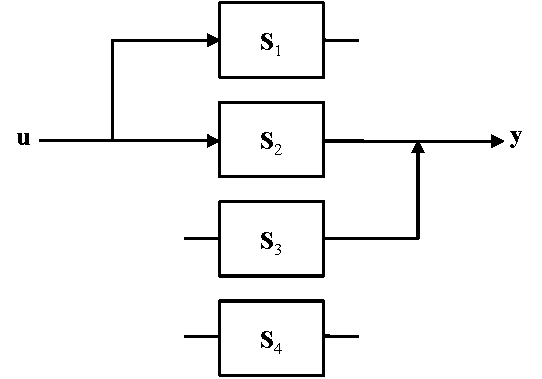
\includegraphics{pictures/partitioning.pdf}}
\end{center}
\endinput

%%% Local Variables: 
%%% mode: latex
%%% TeX-master: "notes"
%%% End:
\end{slide}
\fi

\subsection*{System with Repeated Poles}

If the transfer function has repeated poles, then the form of the
model must be changed. The partial fraction expansion contains
terms of the form \[\frac{r_i}{s-p_i} +
\frac{r_{i+1}}{(s-p_i)^2}.\] This is most easily implemented using
the \emph{Normal Controllable Canonical Form} using a series
connection of the block diagram for the single pole
\[\frac{1}{s-p_i}\] as shown in \sref{slide:l6s4}. By examination
of this diagram it should be clear that the signal seen at point
$A$ is \[A(s) = \frac{r_i}{s-p_i}U(s)\] and that at $B$ is
\[B(s) = \frac{1}{s-p_i}\times\frac{1}{s-p_i}\times r_{i+1} U(s)\] as required.
\begin{slide}\label{slide:l6s4}
\heading{Part of a System with Repeated Poles}
\resizebox{300pt}{!}{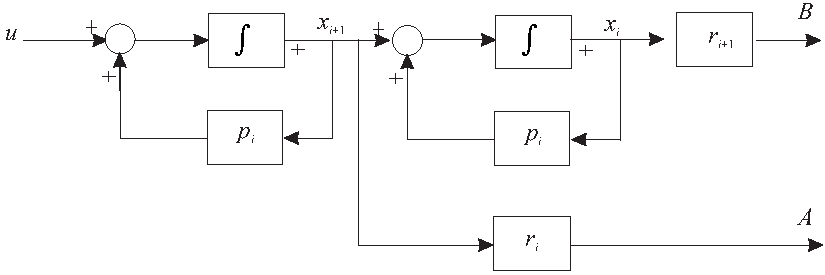
\includegraphics{pictures/jordanblock.pdf}}
\end{slide}
For this portion of the state space model we have
\begin{eqnarray*}
\left[\begin{array}{c}
  \dot{x}_i \\
  \dot{x}_{i+1}
\end{array}\right] &=& \left[\begin{array}{cc}
  p_i & 1 \\
  0 & p_i
\end{array}\right]\left[\begin{array}{c}
  x_i \\
  x_{i+1}
\end{array}\right] + \left[\begin{array}{c}
  0 \\
  1
\end{array}\right] u\\
y & = & \left[r_{i+1},\ r_i\right]\left[\begin{array}{c}
  x_i \\
  x_{i+1}
\end{array}\right].
\end{eqnarray*}

By comparison of this result with the normal situation we see that
the state matrices (of the observer controllable canonical form)
are modified as follows.
\begin{itemize}
  \item in $\mathbf{A}$ \[\left[\begin{array}{cc}
    p_i & 0 \\
    0 & p_{i+1} \\
  \end{array}\right] \rightarrow \left[\begin{array}{cc}
    p_i & 1 \\
    0 & p_{i} \\
  \end{array}\right];\]
  \item in $\mathbf{B}$ \[\left[\begin{array}{c}
    1 \\
    1  \\
  \end{array}\right] \rightarrow \left[\begin{array}{c}
    0 \\
    1 \\
  \end{array}\right];\]
    \item in $\mathbf{C}$ \[\left[\begin{array}{cc}
    r_i & r_{i+1}\\
  \end{array}\right] \rightarrow \left[\begin{array}{cc}
    r_{i+1} & r_i\\
  \end{array}\right].\]

\end{itemize}

The block \[\left[\begin{array}{cc}
    p_i & 1 \\
    0 & p_{i} \\
  \end{array}\right]\] is known as a ``\emph{Jordan Block}''. A
  matrix with one (or more) Jordan Blocks instead of a pure diagonal \[\left[\begin{array}{cc}
    p_i & 0 \\
    0 & p_{i+1} \\
  \end{array}\right]\] is in the ``\emph{Jordan Form}''. The idea
  may be extended to systems with poles of higher multiplicity.
  For example for the case where the multiplicity is 3 as in
  \[\frac{1}{(s-p_i)^3}\] the Jordan Block is  \[\left[\begin{array}{ccc}
    p_i & 1 & 0 \\
    0 & p_{i} & 1 \\
    0 & 0 & p_i
  \end{array}\right].\]

\subsection*{Example} The system with transfer function
\begin{eqnarray*}G(s) &=& \frac{1}{s^3 + 4s^2 + 5s + 2}\\
&=& \frac{1}{(s+1)^2(s+2)} \\ &=& \frac{-1}{s+1} +
\frac{1}{(s+1)^2} + \frac{1}{s+2}.\end{eqnarray*} The normal
canonical form is therefore given by:
\begin{eqnarray*}
\mathbf{A} &=& \left[\begin{array}{ccc}
  -1 & 1 & 0 \\
  0 & -1 & 0 \\
  0 & 0 & -2
\end{array}\right] \mathbf{B} = \left[\begin{array}{c}
  0 \\
  1 \\
  1
\end{array}\right]\\ \mathbf{C} &=& \left[\begin{array}{ccc}
  1 & -1 & 1
\end{array}\right] \mathbf{D} = \left[0\right]
\end{eqnarray*}

\subsection*{Normal Canonical Form with Complex Poles}
A system with complex poles will have a partial fraction expansion
containing terms of the form
\[\frac{\Re\{ r_i\} + j\Im\{ r_i\}}{s - \Re\{p_i\} + j\Im\{p_i\}} + \frac{\Re\{r_i\} - j\Im\{ r_i\}}{s - \Re\{p_i\} - j\Im\{p_i\}} \]
(where the poles and the residuals both appear as complex
conjugate pairs). We cannot implement these directly in state
space form because the state matrices must have real coefficients
to be realisable. However, the complex factors involved can be
combined into a quadratic form and blocks replaced in the normal
canonical form\footnote{The details are left as an exercise.} as
follows:
\begin{itemize}
  \item in $\mathbf{A}$ \[\left[\begin{array}{cc}
    p_i & 0 \\
    0 & p_{i+1} \\
  \end{array}\right] \rightarrow \left[\begin{array}{cc}
    +\Re\{p_i\} & +\Im\{p_i\} \\
    -\Im\{p_i\} & +\Re\{p_i\} \\
  \end{array}\right];\]
  \item in $\mathbf{B}$ \[\left[\begin{array}{c}
    1 \\
    1  \\
  \end{array}\right] \rightarrow \left[\begin{array}{c}
    0 \\
    1 \\
  \end{array}\right];\]
    \item in $\mathbf{C}$ \[\left[\begin{array}{cc}
    r_i & r_{i+1}\\
  \end{array}\right] \rightarrow \left[\begin{array}{cc}
    2\Im\{r_{i}\} & 2\Re\{r_i\}\\
  \end{array}\right].\]
\end{itemize}
\subsection*{Final Example}
 The system with transfer function
\begin{eqnarray*}G(s) &=& \frac{6s+6}{s^2 + 4s + 13}\\
&=& \frac{6(s+1)}{(s+2)^2 + 3^2} \\ &=&
\frac{6(s+1)}{(s+2+3j)(s+2-3j)}
\\ &=& \frac{3-j}{s+2+3j} + \frac{3-j}{s+2-3j}.\end{eqnarray*} The normal canonical form is
therefore given by:
\begin{eqnarray*}
\mathbf{A} &=& \left[\begin{array}{cc}
  -2-3j & 0 \\
  0 & -2+3j
\end{array}\right] \mathbf{B} = \left[\begin{array}{c}
  1 \\
  1
\end{array}\right]\\ \mathbf{C} &=& \left[\begin{array}{cc}
  3-j & 3+j
\end{array}\right] \mathbf{D} = \left[0\right]
\end{eqnarray*}
But this is not realisable so instead we use
\begin{eqnarray*}
\mathbf{A} &=& \left[\begin{array}{cc}
  -2 & -3 \\
  3 & -2
\end{array}\right] \mathbf{B} = \left[\begin{array}{c}
  0 \\
  1
\end{array}\right]\\ \mathbf{C} &=& \left[\begin{array}{cc}
  -2 & -6
\end{array}\right] \mathbf{D} = \left[0\right].
\end{eqnarray*}




%----------------------------------------------------------------
% The end of notes
% ----------------------------------------------------------------
\endinput

%%% Local Variables: 
%%% mode: latex
%%% TeX-master: t
%%% End: 
